\newpage
\section{Midsets Abound}
                                  

In this activity we are going to investigate \textit{midsets}.

\begin{definition}\index{midset}
Given two points $A$ and $B$, their \textbf{midset} is the set of points that are an equal distance away from both $A$ and $B$.
\end{definition}

\begin{prob} 
Draw two points in the plane $A$ and $B$. See if you can sketch the
Euclidean midset of these two points.
\end{prob}

\begin{prob}
See if you can use coordinate constructions to find the equation of
the midset of two points $A$ and $B$. If necessary, set $A = (2,3)$
and $B = (5,7)$.
\end{prob}

\begin{prob}
Now working in city geometry, place two points and see if you can find
their midset.
\[
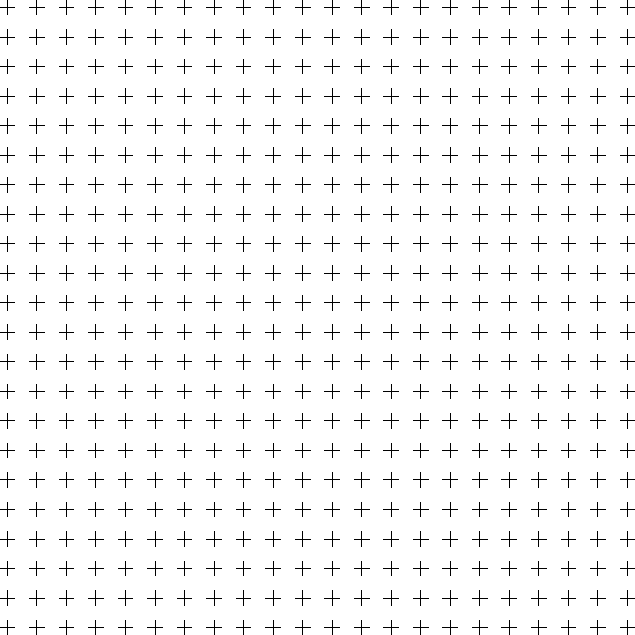
\includegraphics{../graphics/complexPlane}
\]
\end{prob}


\begin{prob}
Let's try to classify the various midsets in city geometry:
\[
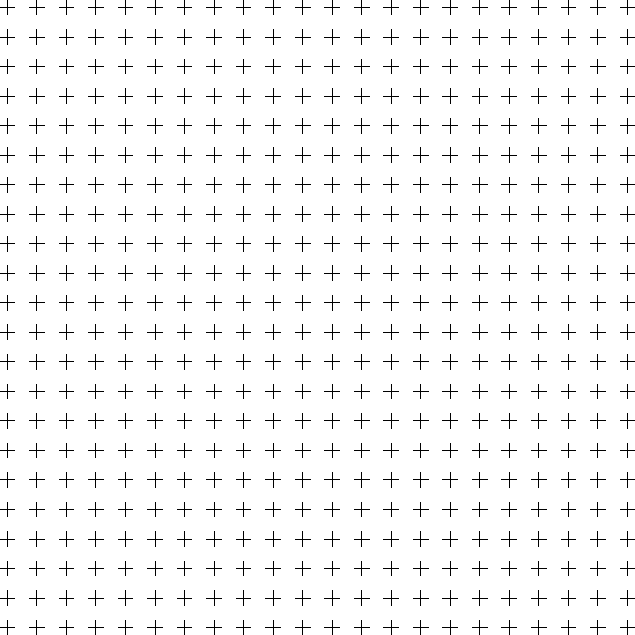
\includegraphics{../graphics/complexPlane}
\]
\end{prob}
